\chapter{车牌识别}
\label{chap:java_ex_recongnition}


手写识别机器学习领域中的一个经典问题。自从深度学习的兴起,MNIST已经是一个被”嚼烂”了的数据集。
该问题要解决的是把28x28像素的灰度手写数字图片,识别为0到9的数字。
而\emph{手写算式识别}在数字识别的基础上,需要识别运算符号,并输出计算结果。

\begin{figure}[!htb]
\centerline{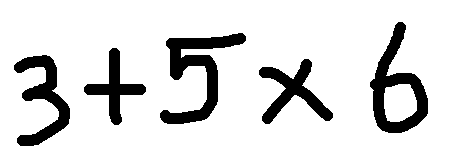
\includegraphics[width=.1\figwidth]{images/handwriting_math.png} $\to$ 识别: $3+5 \times 6$} 
\label{fig:part4_handwriting_math}
\caption{手写算式识别}
\end{figure}

限于篇幅和笔者能力,本演示代码仅支持四则运算($+ - \times \div$),其它运算符号留给同学们研究。
利用深度学习算法,为用户提供手写算式识别,可以极大的提高用户体验。
目前,有很多成熟的产品可以借鉴,相关的论文也非常多。

手写数字识别属于图像分类,可用的算法有:KNN、SVM、BP和CNN。
其中KNN和SVM比较善于数据挖掘,用做手写数字识别的话,比较难达到实用目的;
而BP使用全连接,难于构建深度网络,并存在梯度消失和过拟合问题。
本章例子,选用CNN深度学习训练手写算式识别。

\begin{figure}[!htb] \centering 
\begin{tikzpicture}
\node at (0,0) {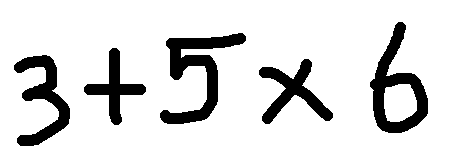
\includegraphics[width=5cm,height=2cm]{images/handwriting_math.png}};
\draw (-2.5,1) rectangle (-1.6,-1);
\draw (-1.6,1) rectangle (-0.8,-1);
\draw (-0.8,1) rectangle (0.3,-1);
\draw (0.3,1) rectangle (1.3,-1);
\draw (1.3,1) rectangle (2.4,-1);
\end{tikzpicture}
\end{figure}

现在我们要识别一个算式,其实和MINIST数字识别没有太多差别,主要是增加了图像切割和四则运算符的识别任务。
为了降低难度,约束字符之间最好有一些间距,不要字符连笔。


\section{图像切割}
手写算式的输入的形式,有2种:拍照、手绘。照片要经过图像处理之后,才能进行切割;
而手绘可直接采集像素轨迹,就省掉了这一步。对于照片的预处理,需要先二值化和降噪把手写数字区域保留下来。
如果考虑图片的背景干扰,可先使用Canny算子检测边缘,这借助OpenCV的API很容易实现。

我们这种要求手写数字不黏连的情况,把Canny输出的图像往X轴投影,就能得出每个数字的横向宽度坐标。
虽然要求数字不黏连,但难保有横向重叠的情况,必须用类似\emph{范水法}进行切割。

\begin{figure}[!htb] \centering 
\begin{tikzpicture}
\node at (0,0) {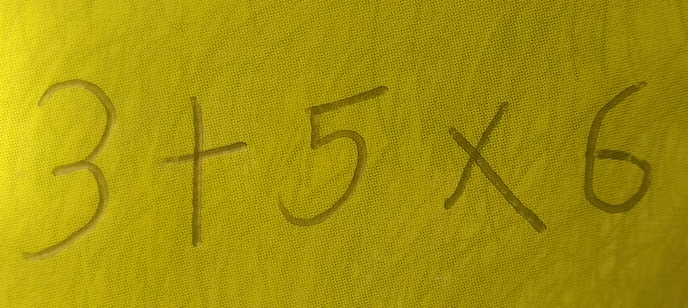
\includegraphics[width=5cm]{images/handwriting_input.png}};
\node at (6,0) {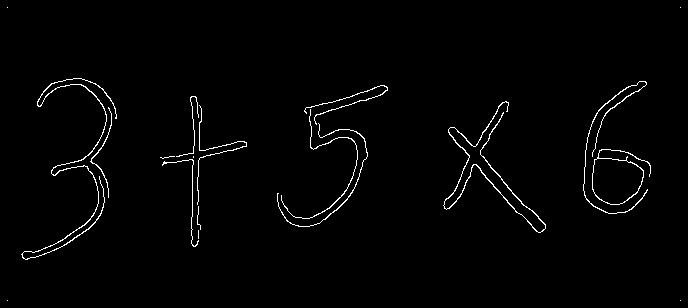
\includegraphics[width=5cm]{images/handwriting_out.png}};
\end{tikzpicture}
\caption{图像处理:二值化和边缘识别(OpenCV)}
\end{figure}

\noindent
这种图像预处理,OpenCV\footnote{OpenCV是一个开源的跨平台视觉库,实现了图像处理和计算机视觉方面的很多通用算法,
支持Linux、Windows、Android和Mac OS操作系统上。
它轻量且高效,同时提供C++、Python、MATLAB等语言的接口。}非常擅长,不需要使用机器学习算法。


\noindent
\emph{Java代码:}
\begin{lstlisting}[language=Java]
System.loadLibrary(Core.NATIVE_LIBRARY_NAME);
Mat img = Imgcodecs.imread(src);
Imgproc.cvtColor(img, img, Imgproc.COLOR_BGR2GRAY);
Imgproc.Canny(img, img, threshold, threshold * 3, 3, true);
Imgcodecs.imwrite(dstImg, img);
\end{lstlisting}

\noindent
\emph{Python代码:}
\begin{lstlisting}[language=Python]
import cv2
from matplotlib import pyplot as plt

img = cv2.imread("handwriting_input.png", 0)
edges = cv2.Canny(img, 30, 60)
plt.subplot(1,2,1), plt.imshow(img, cmap='gray')
plt.title('Original Image'), plt.xticks([]), plt.yticks([])
plt.subplot(1,2,2), plt.imshow(edges, cmap='gray')
plt.title('Edge Image'), plt.xticks([]), plt.yticks([])
plt.show()
\end{lstlisting}

\noindent
实现Canny算子不在本书讨论范围,GitHub上的一份Java实现接近OpenCV的效果
\href{https://github.com/enzoftware/images-processing/blob/master/algorithms/Canny%20Filter/src/com/company/CannyFilter.java}
{\srclink{Github}上获取。}而CSDN上的一份实现简化了很多处理细节,有一定差距。有条件的同学,建议使用OpenCV的接口。
遇到的OpenCV问题,也容易在网络上检索。
\vspace{0.3cm}
\hrule
\begin{multicols}{2}
\begin{itemize}
\item[1.]转换为灰度图像
\item[2.]高斯模糊处理
\item[3.]根据梯度计算图像边缘幅值与角度
\item[4.]非最大信号压制处理(边缘细化)
\item[5.]双阈值边缘连接处理
\item[6.]二值化图像输出结果
\end{itemize}
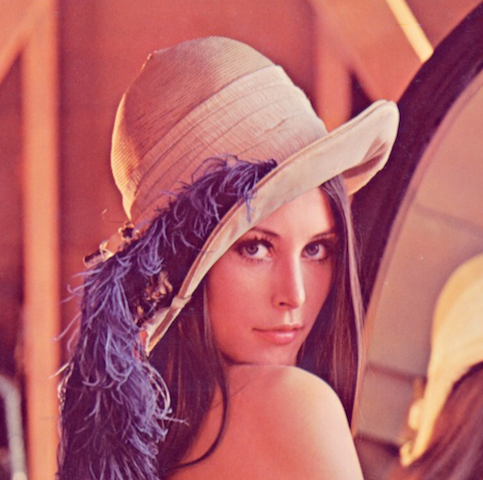
\includegraphics[width=.12\figwidth]{images/Lenna.png}
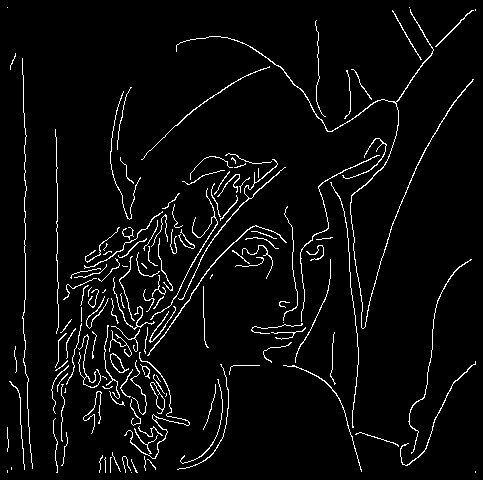
\includegraphics[width=.12\figwidth]{images/Lenna_out.png}
% \end{tabular}
\end{multicols}
\hrule
\ \\
经过Canny算子处理之后,切割图像就非常容易了。把Canny输出的二值图像,在水平方向上投影,对数字进行竖向分割;
同理,在纵向再做一次,就能切割得紧凑一些。以下,是在原图上切割的效果 :

\begin{figure}[!htb] \centering 
\begin{tikzpicture}
\node at (0,0) {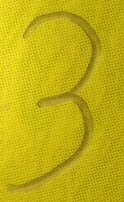
\includegraphics[width=1cm]{images/3.png}};
\node at (2,0) {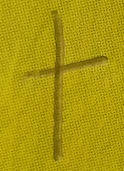
\includegraphics[width=1cm]{images/plus.png}};
\node at (4,0) {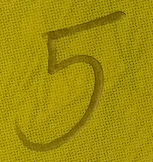
\includegraphics[width=1cm]{images/5.png}};
\node at (6,0) {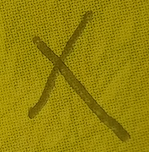
\includegraphics[width=1cm]{images/times.png}};
\node at (8,0) {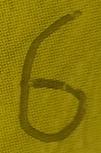
\includegraphics[width=1cm]{images/6.png}};
\end{tikzpicture}
\end{figure}

\noindent
Minist数据集是白底黑字的,使用它训练出来的模型,就很难识别我们的手写算式。所以,有必要在二值图像上切割。
\begin{figure}[!htb] \centering 
\begin{tikzpicture}
\node at (0,0) {
\includegraphics[width=1cm]{images/3_c.png}};
\node at (2,0) {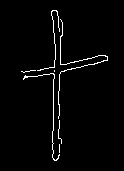
\includegraphics[width=1cm]{images/plus_c.png}};
\node at (4,0) {
\includegraphics[width=1cm]{images/5_c.png}};
\node at (6,0) {
\includegraphics[width=1cm]{images/times_c.png}};
\node at (8,0) {
\includegraphics[width=1cm]{images/6_c.png}};
\end{tikzpicture}
\end{figure}

\noindent
但Canny生成的是空心字,并且有很多断线,使用FloodFill算法是填不满的。
笔者采用的是膨胀法,对于每一个\emph{白色点}向周围扩张6个像素,这样的结果还不错,差不多和Minist数据集很接近了。
\begin{figure}[!htb] \centering 
\begin{tikzpicture}
\node at (0,0) {
\includegraphics[width=1cm]{images/3_b.png}};
\node at (2,0) {
\includegraphics[width=1cm]{images/plus_b.png}};
\node at (4,0) {
\includegraphics[width=1cm]{images/5_b.png}};
\node at (6,0) {
\includegraphics[width=1cm]{images/times_b.png}};
\node at (8,0) {
\includegraphics[width=1cm]{images/6_b.png}};
\end{tikzpicture}
\end{figure}

\noindent
尺寸也要标准化,做成和Minister一样的$28\times28$,这个对图片缩放就可以实现。


\section{算式识别}


\section{结果评估}